% -----------------------------------------------
% Template for ISMIR Papers
% 2026 version, based on previous ISMIR templates

% Requirements :
% * 6+n page length maximum
% * 10MB maximum file size
% * Copyright note must appear in the bottom left corner of first page
% * Clearer statement about citing own work in anonymized submission
% (see conference website for additional details)
% -----------------------------------------------

\documentclass{article}
\usepackage[T1]{fontenc}
\usepackage[utf8]{inputenc}
\usepackage[submission]{ismir} % Remove the "submission" option for camera-ready version
\usepackage{amsmath,cite,url}
\usepackage{enumitem}
\usepackage{graphicx}
\usepackage{color}
\usepackage{booktabs}
\usepackage{multirow}

% Title. Please use IEEE-compliant title case when specifying the title here,
% as it has implications for the copyright notice
% ------
\title{Optical Music Recognition of  Jazz Lead Sheets}

% Note: Please do NOT use \thanks or a \footnote in any of the author markup

% Single address
% To use with only one author or several with the same address
% ---------------
\oneauthor
  {Jiayi Wang \hspace{2cm} Alexander Lerch}
  {Center for Music Technology, Georgia Institute of Technology\\
  \texttt{\{jwang3180, alexander.lerch\}@gatech.edu}}


% Optional: To use hyperref, uncomment the following.
% \usepackage[bookmarks=false,pdfauthor={\authorname},pdfsubject={\pdfsubject},hidelinks]{hyperref}
% Mind the bookmarks=false option; bookmarks are incompatible with ismir.sty.

\sloppy % please retain sloppy command for improved formatting

\def\authorname{J. Wang and A. Lerch}

\begin{document}

\maketitle

\begin{abstract}
Optical music recognition (OMR) of handwritten jazz lead sheets remains a challenging problem due to the variability of chord notation and the limited availability of annotated data. While recent work has shown promising results on pre-segmented system-level lead sheets transcription, full-page handwritten lead-sheet recognition is still unexplored. We present the first full-page OMR system for handwritten jazz lead sheets, adapting the Sheet Music Transformer with a curriculum learning strategy that progressively trains the model on inputs of increasing length, from single systems up to complete pages. To evaluate the system, we construct a detect-and-concatenate pipeline as a full-page baseline and introduce two chord-oriented metrics (Root SER and Chord SER) to assess harmonic transcription quality that standard OMR metrics cannot capture. Experiments show that curriculum training consistently outperforms the baseline, with the largest gains in chord recognition and line level error rate, confirming that page-level context is beneficial for harmonic and structural transcription of jazz lead sheets.
\end{abstract}

\section{Introduction}
Optical Music Recognition (OMR) systems have advanced rapidly in recent years, enabling reliable transcription of printed staff notation into symbolic formats that support useful downstream tasks such as automatic transposition, part extraction, score editing, and computational music analysis. These tools provide meaningful convenience for performers and educators by digitizing traditional sheet music workflows. However, such technology remains underdeveloped for lead sheets, where harmonic symbols serve as the primary medium of musical communication. Unlike fully notated classical scores, jazz lead sheets rely heavily on shorthand, handwritten chord annotations, which are features that challenge existing OMR pipelines designed for printed classical music without chord notation.

Transformer-based architectures such as the Sheet Music Transformer (SMT) have recently demonstrated state-of-the-art performance in printed classical contexts \cite{rios-vila_sheet_2024}, and system-level adaptations for jazz lead sheets show promising results on pre-segmented staff images \cite{martinez-sevilla_optical_2025}. Yet, full-page handwritten jazz recognition remains largely unexplored, particularly with respect to harmonic structure and the preservation of page-level layout.

Chord symbol recognition is the defining challenge of this domain and is fundamentally different from the symbol recognition problems studied in OMR. In jazz, the chord symbols carry the harmonic structure of a song that performers are expected to realize, and any downstream use of a transcribed lead sheet (transposition, search, analysis, accompaniment) depends on correct harmonic content. Yet chord symbols are also the hardest part of the page to read: they are handwritten in shorthand that varies across writers (e.g., \texttt{C$\triangle$7}, \texttt{Cmaj7}, and \texttt{CM7} denote the same chord), they are positioned loosely above the staff rather than aligned to any fixed grid, and they frequently form progressions, like a ii--V--I, that extend across systems. System-level recognition can limit the model’s ability to capture harmonic structures that unfold across multiple systems. Full-page recognition is therefore not just an engineering convenience; by exposing the model to the entire page, it provides an opportunity to leverage broader harmonic context, allowing chord predictions to be informed by surrounding material, and ultimately produce transcriptions that better preserve the structural coherence of a lead sheet.

In this study, We present the first full-page OMR system for handwritten jazz lead sheets, adapting SMT with a curriculum learning strategy that progressively trains the model from single-system inputs up to complete pages. By presenting the entire page simultaneously, the model can condition each prediction on a broader spatial and harmonic context, creating the conditions to learn cross-system dependencies such as chord progressions that span line breaks. Experiments show that this full-page approach yields substantial improvements in structural and harmonic transcription over system-level recognition, with the largest gains in line-level accuracy and chord recognition.
Additionally, we construct a detect-and-concatenate baseline for full-page comparison and introduce two chord-oriented evaluation metrics to assess harmonic transcription quality.

\section{Related Work}
The field of Optical Music Recognition (OMR) research explores computational methods to transcribe images of musical scores to symbolic data (e.g., humdrum, MusicXML, or MEI) \cite{calvo-zaragoza_understanding_2021}. The methodology of OMR has evolved from rule-based, segment detection pipelines to modern deep learning systems. In 2001, early approaches decomposed recognition into staff detection, symbol segmentation, symbol classification, and symbolic reconstruction using statistical or handcrafted features \cite{bainbridge2001challenge}. Later research follows two methodological approaches for full-page transcription. The first focuses on notation object retrieval, where OMR is formulated as a detection problem. These systems locate individual musical primitives before assembling them into a structured representation \cite{devega2022omr,hartelt2022medieval}. The second approach adopts a end-to-end deep learning system: models directly generate a symbolic sequence from the input image without explicit segmentation \cite{alfaro-contreras2023homophonic,rios-vila_sheet_2024}.

Both of these methods have faced two major problems: handwritten score recognition and piano polyphonic transcription. In tackling the handwritten score recognition challenge, deep learning systems have advanced the classical sequence-learning systems:
In 2019, Baró proposed a full HMR (Handwritten Music Recognition) system driven by Convolutional Recurrent Neural Networks \cite{baro_optical_2019}. His appoarch emphasizes data augmentation and transfer learning to cope with handwriting variability, thereby moving beyond stage-specific detectors toward holistic recognition. Concurrent work by Calvo-Zaragoza applied CRNN-CTC to handwritten music notation, decreasing the symbol-level error rate from the baseline for handwritten Mensural notation \cite{calvo-zaragoza_handwritten_2019}. For the problem of polyphonic piano music, Mayer et al. argue that inconsistent symbolic ground truth results in meaningless evaluation and introduce Linearized MusicXML (LMX) to provide a stable, lossless text target for end-to-end models \cite{mayer_practical_2024}. Rios-Vila et al. introduce the Sheet Music Transformer (SMT), an autoregressive image-to-sequence model that directly emits Humdrum **kern encodings, positioning itself as the first end-to-end OMR to tackle complex polyphonic structures\cite{rios-vila_sheet_2024}. 

Unlike classical polyphonic scores, jazz lead sheets combine a monophonic melody with chord symbols, introducing a structure and vocabulary that remain underexplored in OMR. Martínez-Sevilla et al. present the first dataset and system for this task, adapting SMT to transcribe pre-segmented staff images~\cite{martinez-sevilla_optical_2025}. While recent work begins to address this domain, evaluating harmonic transcription quality remains challenging, as standard OMR metrics do not fully capture the role of chord symbols. At the same time, the system-level formulation leaves open how models can learn relationships that extend beyond individual systems, particularly for harmonic structures such as chord progressions that span line breaks. In this work, we investigate full-page recognition as a means to expose broader structural and harmonic context across systems.

\section{Methodology}
To investigate these questions, we adapt Shee Music Transformer(SMT) model to take a full page as input and directly produce a complete humdrum transcription spanning all systems, without any intermediate segmentation step. Given a grayscale scan of a full page of music, the goal is to produce a complete humdrum transcription that encodes both the melodic content and the chord symbols.


\subsection{Dataset}
We adopt the Jazzmus dataset~\cite{martinez-sevilla_optical_2025}, a collection of jazz lead sheets consisting of handwritten and synthetic scores aligned with Humdrum and MusicXML encodings. The dataset provides two versions: individual staff system crops (1,688 train / 105 val / 228 test) and complete full-page scans (245 train / 16 val / 32 test). The synthetic portion includes 326 full-page renderings (with its system level version) generated using MuseScore with two font styles (Classical and MuseJazz) to approximate real-world variability. The handwritten portion includes 293 pages (163 unique works) produced by jazz professionals and students who manually copied the synthetic lead sheets. All multiple copies of the same piece are restricted to the training set, preventing leakage of identical musical content across splits.

The Jazzmus annotations are derived from MusicXML-to-Humdrum \texttt{**kern} conversion, and we apply a data cleaning to improve consistency for training. First, chord symbols in the \texttt{**mxhm} spine that were occasionally represented as comment instead of chord annotations, which makes the model ignore those chords. Second, for the synthetic subset, we correct system-level bounding boxes to ensure that each staff crop consistently includes the corresponding chord annotations above the staff. These refinements are contributed back to the dataset though submitting hugging face pull request. Additionally, the handwritten portion reflects natural variation introduced during manual copying of lead sheets. Minor discrepancies, such as differences accidentals and slur markings, may appear between the image and the symbolic annotation. We retain these variations as part of the dataset, as they provide a realistic setting for evaluating model robustness to handwritten input.


% should this be discussed here? or leave to the later curriculum training stragety to explain
To train the full-page model, we investigate two data preparation strategies for curriculum learning.
In the masking approach, each full page is prepared as a set of progressive crops containing the top $N = 1, \ldots, 9$ systems, so the model is trained on real page content of increasing length.
In the stacking approach, a synthetic training set is generated offline by vertically concatenating $N$ randomly selected system images into a single multi-system image, for $N = 1, \ldots, 9$, providing greater training diversity by combining systems from different pieces.

For multi-system inputs, ground-truth files are assembled by concatenating per-system annotations. The first system retains the file header and spine declarations, subsequent systems have their headers removed, and systems are joined using \texttt{!!linebreak:original} separators. The final system retains the spine terminators (\texttt{*-}). This convention is applied consistently across data preparation, training, and evaluation.

\subsection{Model Architecture}
We adopt the Sheet Music Transformer (SMT)~\cite{rios-vila_sheet_2024}, an encoder–decoder architecture for image-to-sequence music transcription. SMT uses a convolutional encoder (ConvNeXt) to extract visual features from the input image and a Transformer decoder to autoregressively generate a Humdrum token sequence via cross-attention. To adapt SMT to the full-page setting, we extend the output vocabulary with a \texttt{<linebreak>} token, allowing the model to explicitly represent system boundaries and generate multi-system transcriptions.


\subsection{Baseline: System-Level Recognition with YOLO Segmentation}
To establish a full-page comparison point, we construct a detect-and-concatenate pipeline: a staff detector locates individual systems on the page, each system is transcribed independently by the system-level SMT model, and the predictions are concatenated into a full-page output.
This pipeline is designed for this paper to measure how far a detect-and-concatenate approach can go without any page-level training.

\subsubsection{Staff Segmentation}
Page images are first preprocessed with resize and de-skewed method to correct size and rotations.
We adopt YOLO detector~\cite{dvorak2024staff} fine-tuned on the music staff-detection task then detect bounding boxes for each staff system.
Raw detections are post-processed in three steps.
First, the raw detection boxes only cover the staff lines and notes, leaving chord symbols that appear above the staff uncaptured; to address this, non-overlapping crop boundaries are extended by splitting each inter-system gap 75/25, allocating the larger share upward so that chord notation above each staff is fully included in the crop.
Second, inter-system gaps are analyzed to recover missed detections: the median gap between adjacent systems is used as a reference stride, and any gap exceeding 2$\times$ the median triggers the insertion of one or more virtual bounding boxes by linear interpolation between the surrounding systems.
Third, duplicate detections of the same staff are removed by computing overlapping area between every pair of boxes and retaining one box when there is a duplicate detection.
The first and last systems use the average gap as padding rather than extending to the page edge.

\subsubsection{System-Level Recognition}
Each cropped system image is fed to the SMT model pretrained on the system level study \cite{martinez-sevilla_optical_2025}.
The per-system predictions are concatenated into a full-page output: the first system's header and spine declarations are preserved, subsequent systems have their humdrum headers stripped, and all systems are joined with line-break notation in humdrum (\texttt{!!linebreak:original}) separators, with spine terminators appended at the end.


\subsection{Curriculum Training}

To bridge the gap between the system-level model and full-page recognition, we investigate two curriculum learning strategies that progressively expose the model to longer, more complex inputs.

\subsubsection{Masking Curriculum}

The masking curriculum starts from the pretrained system-level SMT checkpoint and progressively exposes it to longer page excerpts drawn from real full-page scans.
For each full-page scan, we derive a family of training crops by retaining only the top $N$ systems and cropping away the rest, for $N = 1, \ldots, 9$.
The 1-system crop is identical to a standard system-level input, while each subsequent crop adds one more system, creating a natural progression of difficulty that exposes the model to progressively longer and more complex page-level sequences.
We use 9 stages because most pages contain 7--8 systems; pages with 9 or more systems are rare enough that stages 9--11 are merged into a single final stage.
The corresponding ground-truth sequence for each $N$-system crop is assembled by concatenating per-system annotations using the header-stripping and \texttt{!!linebreak:original} separator convention described in the dataset section.

Training proceeds through the curriculum in sequential stages.
At stage $k$, only crops with $N \leq k$ are eligible for sampling, so each stage introduces one additional system beyond the previous stage's maximum.
The stage advances automatically once the validation SER falls below a fixed threshold for a number of consecutive validation epochs, ensuring that the model has adequately learned the current input length before moving on.
At the final stage ($k = 9$), each page contributes its full crop and training continues under an early-stopping criterion until validation no longer improves.

A direct consequence of this staged training regime is that when the distribution shifts from stage $k-1$ to stage $k$, samples from earlier stages disappear from the loss entirely, and the model can catastrophically forget shorter-input behavior it previously learned.
To mitigate this, we apply experience replay: at stage $k$, a fraction $r$ of samples from each prior stage $s < k$ is randomly drawn and added to the current training pool, where for stage $s$ we sample $\max(1, \lfloor r \cdot |\mathcal{D}_s| \rfloor)$ items.
The replay ratio $r$ thus controls the tradeoff between specialization to the current stage and retention of prior stages; its effect is studied as an ablation in Section~\ref{sec:results}.

\subsubsection{Stacking Curriculum}

The stacking curriculum removes the dependency on pre-existing multi-system page crops by synthesizing multi-system training images directly from the much larger pool of individual system crops.
For each stage $N = 2, \ldots, 9$, a training image is constructed by vertically stacking $N$ individual system images: a random anchor system is drawn from the training set, and $N-1$ additional systems are sampled from its width-compatible pool so that the resulting composite is geometrically consistent.
All selected systems are resized to a uniform height with aspect ratio preserved, padded to a common width, and vertically concatenated into a single image.
The corresponding ground-truth sequence is assembled by concatenating per-system annotations following the header-stripping and \texttt{!!linebreak:original} separator convention described in the dataset section.
Because any combination of width-compatible systems can be stacked, this construction yields a combinatorially much larger set of unique $N$-system examples than the masking curriculum, which is bounded by the number of real pages.

Training proceeds through the same staged advancement mechanism as the masking curriculum: stage $N$ restricts sampling to stacks of at most $N$ systems, advances when the validation SER threshold is met, and applies experience replay from prior stages to mitigate catastrophic forgetting.
Stage $N = 1$ requires no stacking: the system-level entries from Jazzmus are used directly, which also allows the model to be trained from scratch on genuine system-level data before progressing to stacked compositions.
At the final stage ($N = 9$), real full-page scans are appended to the training pool so that the model observes authentic page-level layout, closing the gap between the synthetically stacked training distribution and the real full-page test distribution.

\subsection{Evaluation Metrics}

We report five metrics, all computed as Levenshtein edit-distance error rates.
Following standard OMR practice, we report Character Error Rate (CER), Symbol Error Rate (SER), and Line Error Rate (LER), which measure recognition accuracy at the character, symbol, and row levels respectively.
These three metrics are also computed on the **kern spine only, isolating note-level transcription quality from chord recognition so that melodic and harmonic errors can be assessed independently.
SER is additionally used as the primary signal for curriculum stage advancement.

Chord recognition is a task unique to jazz lead sheets: unlike classical OMR, where the score encodes only melody and rhythm, jazz lead sheets explicitly notate harmonic symbols that are central to performance and analysis.
Because no prior OMR evaluation framework addresses chord symbols, standard metrics applied to the full humdrum output cannot isolate harmonic errors from melodic ones.
We therefore introduce two chord-oriented metrics computed solely from the \texttt{**mxhm} spine:
\begin{itemize}[leftmargin=*]
\item \textbf{Root SER}: extracts only the root-note token from each chord symbol and computes the Levenshtein distance between the predicted and ground-truth root sequences, normalized by the total number of ground-truth root tokens. It isolates errors in fundamental pitch recognition.
\item \textbf{Chord SER}: extracts the full chord token (excluding duration dots) and applies the same edit-distance computation, penalizing errors in chord quality and extensions beyond the root.
\end{itemize}
Both metrics are computed at the page level by pooling edit-distance counts across all pages before normalizing.


\section{Experimental Setup}

All experiments are evaluated on the 32-page full-page test set and run on a single NVIDIA H200 GPU with BF16 mixed precision.

\subsection{Baseline}
The baseline requires no training; it applies the pretrained system-level SMT checkpoint directly to YOLO-detected crops and concatenates the per-system predictions into a full-page output.

\subsection{Masking Curriculum}
The 245 real and 278 synthetic full-page training scans each contribute up to 9 crops, yielding 4,707 training entries; validation uses the corresponding 288 crops from 16 real full-page scans.
SMT is initialized from the pretrained system-level checkpoint with the output head extended to include the \texttt{<linebreak>} token, and optimized with AdamW ($lr = 5 \times 10^{-6}$, 150 warmup steps), with validation every 10 epochs.
A batch size of 8 is used for stages 1--8; at stage 9, the batch size is reduced to 1 due to GPU memory constraints imposed by full-page inputs.
The stage-advancement SER threshold is set to 20\% with a patience of 5 consecutive validation epochs; at the final stage, early stopping triggers after 10 epochs without improvement.
To study the effect of experience replay, we run four variants with replay ratio $r \in \{0, 0.25, 0.50, 1.00\}$.

\subsection{Stacking Curriculum}
For stage $N = 1$, the 1,688 real and 1,872 synthetic system-level entries from Jazzmus are used directly.
For stages $N = 2, \ldots, 9$, we generate 1,688 real-stacked and 1,872 synthetic-stacked images per stage (system height 256\,px), maintaining real-to-synthetic balance throughout, yielding 32,563 training entries across all stages with 856 validation entries.
At stage 9, the 245 real and 278 synthetic full-page images are additionally appended to the training pool.
SMT is trained from scratch ($lr = 1 \times 10^{-5}$, batch size 8) with replay ratio $r = 0.25$, a stage-advancement SER threshold of 25\% with a patience of 3 validation epochs, and a final-stage early-stopping patience of 10.
To maximize throughput on smaller inputs, gradient accumulation of 2 is applied for stages 2--5 (effective batch size 16), reverting to batch size 8 for stages 6--8.



\section{Results}
\label{sec:results}

\subsection{Baseline}

The detect-and-concatenate baseline achieves 13.55\% CER, 12.78\% SER, and 32.35\% LER on the 32-page test set (Table~\ref{tab:overall}).
While token-level accuracy is reasonable, the high LER indicates that structural errors accumulate when independently transcribed systems are concatenated without shared positional context.
Spine-specific evaluation (Table~\ref{tab:spine}) reveals that chord recognition is disproportionately difficult: the baseline achieves 14.40\% kern SER but 47.82\% Chord SER and 29.17\% Root SER, confirming that harmonic symbols pose a greater challenge than melodic content.

\begin{table}[t]
\centering
\caption{Overall full-page recognition results on the 32-page test set. All values are edit-distance error rates (\%; lower is better).}
\label{tab:overall}
\renewcommand{\arraystretch}{1.15}
\begin{tabular}{lrrr}
\toprule
\textbf{Method} & \textbf{CER} & \textbf{SER} & \textbf{LER} \\
\midrule
Baseline              & 13.55 & 12.78 & 32.35 \\
Masking, $r=1.00$     & 13.32 & 12.50 & 23.15 \\
Stacking              & \multicolumn{3}{c}{\textit{pending}} \\
\bottomrule
\end{tabular}
\end{table}

\subsection{Masking Curriculum}

Table~\ref{tab:spine} reports spine-specific metrics across all four replay variants.
Without replay ($r=0$), kern-only CER and SER degrade relative to the baseline (17.20\% vs.\ 11.96\% and 18.39\% vs.\ 14.40\%), indicating that na\"ive curriculum training without replay causes catastrophic forgetting.
However, even without replay, kern-only LER remains comparable to the baseline (26.62\% vs.\ 26.66\%), suggesting that structural line-level accuracy is preserved even when token-level quality suffers.
Performance improves monotonically with increasing replay ratio.
With full replay ($r=1.00$), kern-only metrics improve across the board: CER drops to 11.63\%, SER to 13.02\%, and LER to 18.67\%, all surpassing the baseline.
The largest relative gains appear in the chord-specific metrics: Chord SER falls by 35.9\% (47.82\% to 30.67\%) and Root SER by 27.2\% (29.17\% to 21.25\%) compared to the baseline, confirming that page-level harmonic context is particularly informative for chord quality and extension disambiguation.

On the overall metrics (Table~\ref{tab:overall}), the masking curriculum with full replay yields modest improvements on CER (13.32\% vs.\ 13.55\%) and SER (12.50\% vs.\ 12.78\%), but LER drops substantially from 32.35\% to 23.15\%.
The contrast between modest CER/SER improvements and substantial gains in LER and chord metrics suggests that the primary benefit of full-page training lies in structural coherence across line boundaries and harmonic context, rather than finer-grained symbol recognition.

\begin{table}[t]
\centering
\caption{Spine-specific metrics on the 32-page test set across masking replay ratios. Kern-only metrics are computed on the \texttt{**kern} spine; Root and Chord SER on the \texttt{**mxhm} spine. All values are error rates (\%; lower is better).}
\label{tab:spine}
\renewcommand{\arraystretch}{1.15}
\resizebox{\columnwidth}{!}{%
\begin{tabular}{lrrrrr}
\toprule
\textbf{Method} & \textbf{Kern} & \textbf{Kern} & \textbf{Kern} & \textbf{Root} & \textbf{Chord} \\
                & \textbf{CER}  & \textbf{SER}  & \textbf{LER}  & \textbf{SER}  & \textbf{SER}   \\
\midrule
Baseline              & 11.96 & 14.40 & 26.66 & 29.17 & 47.82 \\
\midrule
Masking, $r=0$        & 17.20 & 18.39 & 26.62 & 26.39 & 39.16 \\
Masking, $r=0.25$     & 15.08 & 16.12 & 22.31 & 26.31 & 37.59 \\
Masking, $r=0.50$     & 14.10 & 15.68 & 22.18 & 23.36 & 35.70 \\
Masking, $r=1.00$     & 11.63 & 13.02 & 18.67 & 21.25 & 30.67 \\
\midrule
Stacking              & \multicolumn{5}{c}{\textit{pending}} \\
\bottomrule
\end{tabular}%
}
\end{table}

\subsubsection{Effect of Experience Replay}

\begin{figure}[b]
\centering
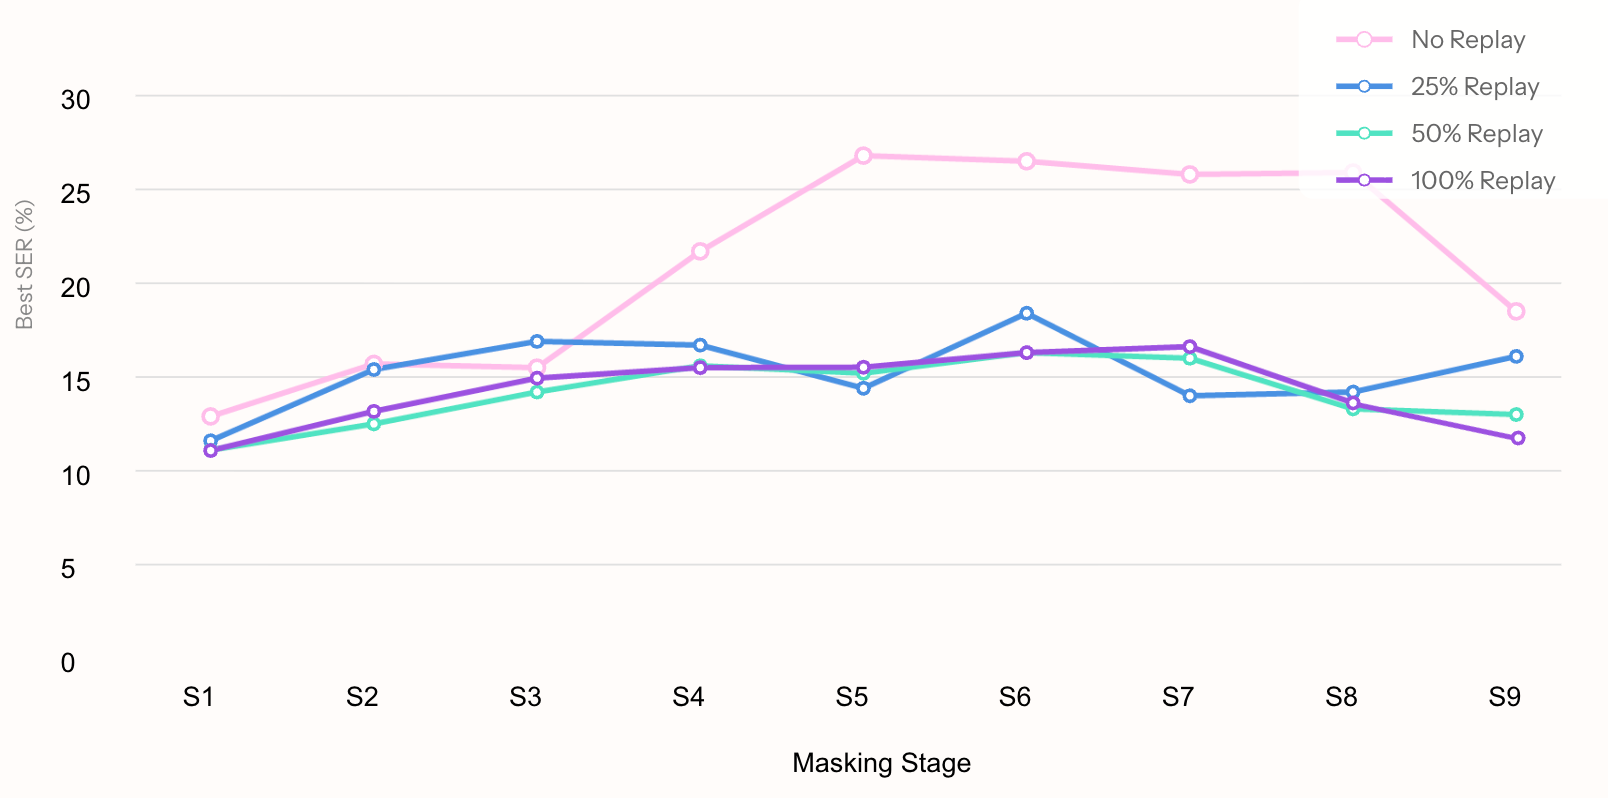
\includegraphics[width=\columnwidth]{Msking stage validation comparison.png}
\caption{Best validation SER (\%) at each masking curriculum stage (S1--S9) for four experience replay ratios. Without replay, SER spikes sharply at mid-stages due to catastrophic forgetting. Increasing the replay ratio stabilizes performance across all stages.}
\label{fig:masking_stages}
\end{figure}

To understand the mechanism behind the test-set differences, we examine the best validation SER achieved at each curriculum stage (Figure~\ref{fig:masking_stages}).
Without replay, SER rises sharply from S4 to S6, peaking at approximately 27\%, as the model overwrites its knowledge of shorter inputs when the training distribution shifts to longer sequences.
With 25\% and 50\% replay the curve is substantially flatter, though mid-stage performance still degrades relative to earlier stages.
At 100\% replay, SER remains stable throughout all nine stages and converges to the lowest value at S9.
The monotonic relationship between replay ratio and stage-level stability directly explains the test-set trends in Table~\ref{tab:spine}: higher replay produces not only better final performance but more consistent learning throughout the curriculum.

\subsection{Stacking Curriculum}

Results for the stacking curriculum are pending and will be reported upon completion.


\section{Discussion}
\label{sec:discussion}


\subsection{Why full-page recognition matters}
The detect-and-concatenate baseline achieves competitive CER and SER, showing that system-level transcription already captures most token-level content accurately.
Yet the same baseline exhibits higher LER (32.35\%) and Chord SER (47.82\%), revealing that the errors it does make disproportionately affect structural and harmonic elements.

This pattern is expected: a model that reads one system at a time has no access to the chord progressions, phrase boundaries, or key context established in earlier systems.
Chord symbols in jazz lead sheets are inherently sequential across systems. For example, a ii--V--I progression that spans a line break is split into disconnected fragments when each system is transcribed independently.
Similarly, LER penalizes line-level insertions and deletions that arise when the concatenation pipeline must reconstruct page structure from independently predicted outputs without any shared positional information.

Full-page recognition addresses both limitations by presenting the entire page simultaneously, allowing the model to condition each prediction on the full spatial and harmonic context.
The results confirm this: with full replay, Chord SER drops by 35.9\% (47.82\% to 30.67\%) and LER by 28.4\% (32.35\% to 23.15\%), while CER and SER improve only marginally.
The kern-only metrics tell the same story from the melodic side --- kern LER improves from 26.66\% to 18.67\%, a 30.0\% relative reduction, while kern CER and SER show modest gains.
This consistent pattern across both spines indicates that the primary benefit of full-page training is not finer-grained symbol recognition but improved structural coherence: the model better understands where systems begin and end, how musical content flows across line breaks, and how harmonic context propagates through the page.

\subsection{Replay is essential for curriculum stability}
The sharp degradation observed at $r=0$ reveals that curriculum training can be counterproductive without a mechanism to retain prior knowledge.
In the masking setting, the training distribution shifts abruptly at each stage boundary: training samples at stage $k-1$ disappear entirely from the loss at stage $k$ unless replayed in the training data.
As shown in Figure~\ref{fig:masking_stages}, this causes validation SER to spike at mid-stages, reaching approximately 27\% at S5--S6 before partially recovering.
Experience replay acts as a regularizer that keeps earlier stage distributions present throughout training.
The monotonic improvement with increasing $r$ across all metrics in Table~\ref{tab:spine} suggests that the full dataset history ($r=1.00$) is not yet redundant, and retaining all prior data continues to benefit performance even at the final stage.

\subsection{Chord metrics as a diagnostic tool}
Standard OMR metrics such as SER and CER aggregate errors across all tokens equally, diluting errors in chord symbols that are sparse relative to the melodic token stream.
Root SER and Chord SER isolate the harmonic layer and reveal a gap that CER/SER alone would understate: the baseline achieves 12.78\% SER but 47.82\% Chord SER, indicating that chord recognition is disproportionately difficult even when overall symbol accuracy is acceptable.
This argues for routinely reporting chord-specific metrics in jazz OMR evaluations, as they expose model weaknesses that aggregate metrics obscure.

\subsection{Stacking vs.\ masking}
The masking curriculum relies on existing full-page scans to construct its training crops, limiting the number of distinct $N$-system examples to the size of the page collection.
The stacking curriculum removes this bottleneck by synthesizing training images from individual system crops, generating thousands of unique $N$-system combinations per stage while maintaining a real-to-synthetic balance throughout.
Whether this diversity advantage translates to better generalization on real full pages is an open question that the pending stacking results will address.


\section{Conclusion}

We have presented the first full-page OMR system for handwritten jazz lead sheets, comparing a detect-and-concatenate baseline with two curriculum learning approaches that progressively train the model on inputs of increasing length.
The masking curriculum with full experience replay ($r=1.00$) outperforms the baseline on all evaluation metrics, with the most pronounced improvements in LER (32.35\% to 23.15\%) and Chord SER (47.82\% to 30.67\%), confirming that page-level context is beneficial for structural and harmonic transcription.

A key insight is that experience replay is not merely helpful but necessary: without it, curriculum training degrades performance relative to the baseline, and error rates decrease monotonically as more prior-stage data is retained.
The introduction of chord-specific evaluation metrics (Root SER and Chord SER) also proved valuable, surfacing harmonic recognition errors that aggregate token-level metrics systematically understate.

As noted in Section~3.1, the annotation-performance mismatch introduced by the data cleaning process represents an irreducible noise floor; disentangling transcription errors from annotation inconsistencies is an important direction for future work.

More broadly, data scarcity remains the primary bottleneck: the Jazzmus dataset contains only 293 handwritten pages, limiting both training diversity and evaluation reliability.
A natural next step is to construct a larger corpus by re-engraving standards from the Real Book with kern annotations and collecting corresponding handwritten copies, which would provide both greater scale and cleaner ground truth.
Existing kern-encoded jazz corpora such as the Charlie Parker Omnibook transcriptions used in~\cite{baker_idiomaticism_2016} could serve as a starting point for building such a resource.
Finally, vision-language models (VLMs) pretrained on large-scale image-text data offer a promising alternative to training OMR systems from scratch; exploring transfer learning from VLMs to music score recognition could reduce the dependence on domain-specific annotated data and improve generalization to unseen handwriting styles.

\section{Acknowledgements}
This work used the Partnership for an Advanced Computing Environment (PACE) at the Georgia Institute of Technology (RRID:SCR\_027619).

% For BibTeX users:
\bibliography{OMR}


\end{document}


% some notes about the lerch meeting:
% flow chart can be two different thing with one on baseline inference and the other on training
% think about the maybe construct the replay ratio as a ablation or differenet experiment
% maybe some of the data prep can be in the experiment setup section
% Pace acknoleagement goes to acknowleagemenbt section
% maybe bar graph for the tables?
% discussion and result think about that 